%-------------------------------------------------------------------------------
\section{Motivation}\label{motivation}
%-------------------------------------------------------------------------------

We now explore a little more the benefits that serverless has to offer, the
current state of the world, and how our approach fits in with both of these.

\subsection{Benefits of serverless}

The main attraction is, in an idealized world, the characteristic of only paying
for what you use while having a whole datacenter available to you. This is
especially attractive to developers of applications where the amount of
resources that they need varies significantly over time, or is generally small
and very spread out, so that buying their own machines or renting a fixed amount
doesn't suit their actual needs well.

A central example to this paper is that of a web server. Its traffic patterns
make it a great candidate for running entirely as serverless jobs: it is
event-based, its load is bursty and unpredictable, and a request's resource
requirements can vary greatly depending on which user invoked it.


Some back of the envelope math shows that for web servers with small load,
Lambda functions as they stand today are cheaper: for a low-traffic website,
with approx 50K requests per day, a memory footprint of < 128 MB, and 200ms of
execution, running that on AWS lambda adds up to \$1.58 per month. On the other
hand, the cheapest EC2 instance costs just over \$3 per month. Of course, as the
number of requests goes up, the price for lambdas scales linearly, whereas
running an EC2 instance on full load becomes comparably cheap. There are pretty
extensive simulations that others have done that show the tradeoff points for
different types of workloads.
% https://www.bbva.com/en/innovation/economics-of-serverless/
% https://www.trek10.com/blog/lambda-cost

Serverless also may outperform reservation systems for workloads that are very
bursty: starting a new lambda execution environment is much faster than starting
a new container or EC2 instance, which can take multiple minutes.
% https://docs.aws.amazon.com/autoscaling/ec2/userguide/ec2-auto-scaling-default-instance-warmup.html 


\subsection{State of the world}


\begin{figure}[t!]
    \centering
      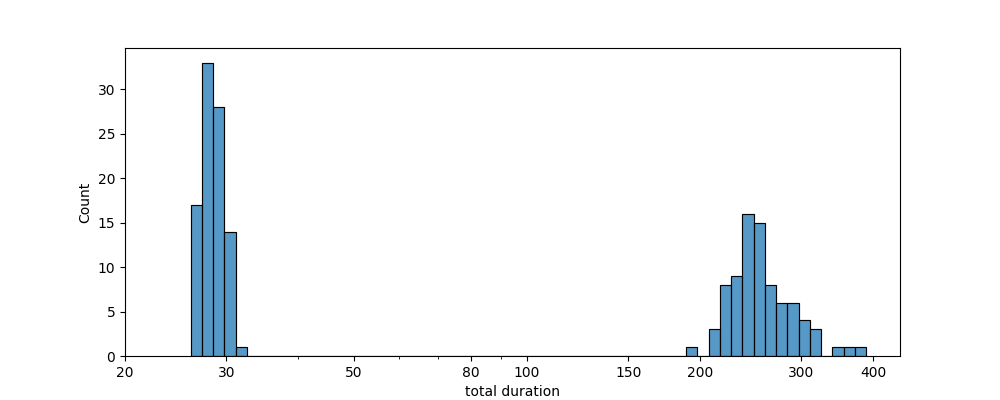
\includegraphics[width=8.5cm]{img/lambda_total_durations.png}
      \caption{ add caption }
    \label{fig:lambda-total-durations}
\end{figure}

However, only few web servers actually run entirely on serverless offerings
today. There are many reasons that developers choose not to use serverless,
despite in theory having workloads that are well-suited for the serverless
environment.
% https://www.reddit.com/r/aws/comments/yxyyk3/without_saying_its_scalable_please_convince_me/
Popular complaints include provider lock in, lack of insight for debugging and
telemetry, and variable runtimes.


We focus on what is arguably the most fundamental of these complaints; which is
the variable runtimes. We run a small experiment with a hello world style lambda
function that simply sleeps for 20ms and measure its end to end latency, with
incovations spaced randomly between 0 and 10 minutes to ensure a fair spread of
warm and cold start. The results are in Figure~\ref{fig:lambda-total-durations}.
The left hand side of the graph is clearly the execution times from warm start,
which remain fairly stable. Reason for this is likely that AWS is able to simply
route the new request to the machine with the existing container on it, although
we still see a small variance of $\sim$10ms. The left hand side of the graph is then
the cold start times, which vary between 200 and 400ms. What this side of the
graph tells us is that when a request encounters cold start, the variability in
latency goes up a lot. 

\begin{figure}[t!]
  \centering
    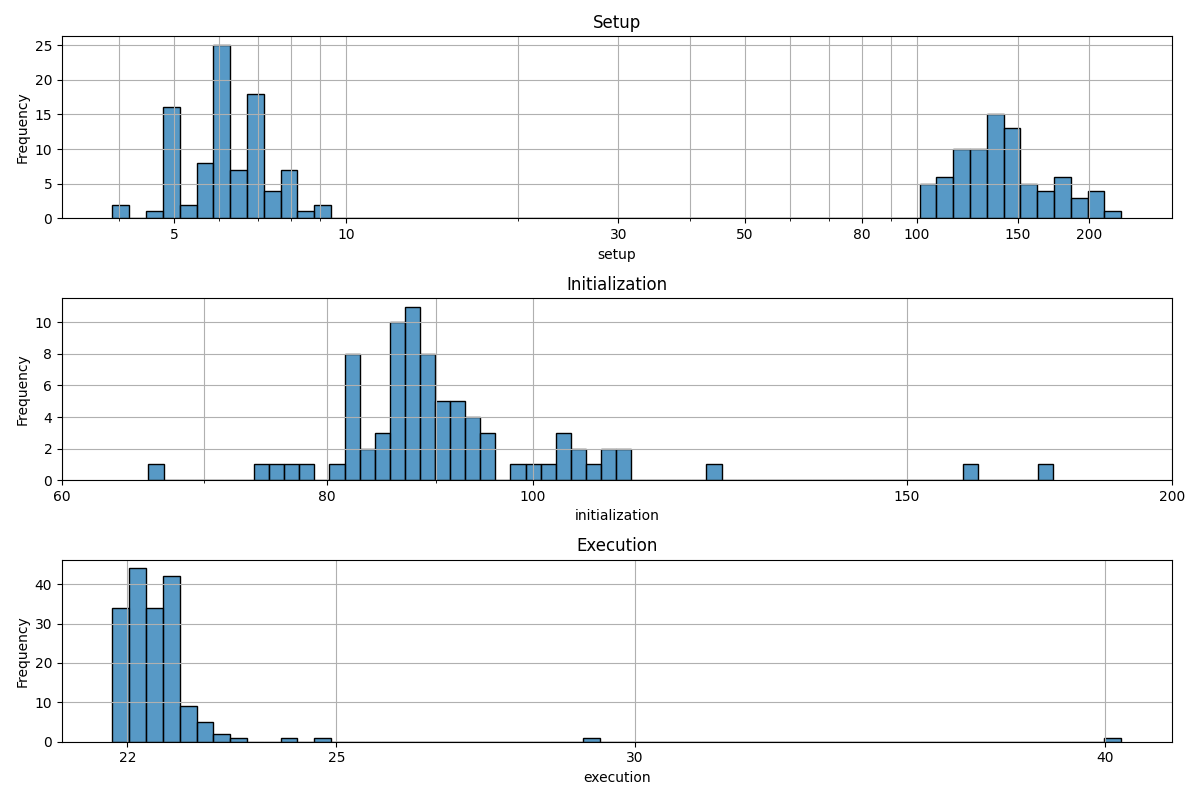
\includegraphics[width=8.5cm]{img/lambda_duration_breakdown.png}
    \caption{ add caption }
  \label{fig:lambda-durations-breakdown}
\end{figure}

In order to better understand where that variabillity comes from, we look into a
breakdown of the latencies using AWS' Xray tracing. 
% https://aws.amazon.com/xray/
We are able to break down the total duration into three components:
\textit{setup}, which includes placing the function and creating the container;
\textit{initialization}, which includes initializing the runtime, and any
extensions the function uses; and \textit{execution}, actually executing the
functions code. Xray only gives us the latter two values explicitly, we
calculate the setup time by looking at the total duration and subtracting the
initalization and execution times. We see the resulting distributions in
Figure~\ref{fig:lambda-durations-breakdown}. TODO do analysis here


\hmng{TODO we need a transition here ... or we do we even still want the part that
comes next? I do think talking about the interface is good though}

The information that AWS gets about the functions it needs to run is an amount
of memory, which is then tied to a cpu power (an amount of vCPUs). However,
memory usage is at best difficult to know in advance and at worst has a large
variance so is impossible to say in advance, and more importantly is not
correlated with what developers actually care about, which is job latency. In
fact, measurements have shown that in some ways the two are inversely
correlated, ie that lambdas that had more memory allocated took longer to start
up. 
% https://www.simplybusiness.co.uk/about-us/tech/2019/03/aws-lambda-cold-start/. 

